\section{Introduction}
Todays usage of wireless networks grows dramatically. The increase in mobile phone usage as well as mobile digital communication implies a lot of challenges to hardware and software designs and opens up new areas of academic research. The variety of 802.11 standards shows the growing complexity of mobile technologies. Still many of the problems being faced with in mobile technologies are very basic and show how even the most obvious solutions can be improved.

RF\footnote{Radio Frequency} transmission can be interfered in very many ways. The following parameters can be affected (see \cite{kassner}):

\begin{itemize}
\item \emph{Received signal strength}: Depending on the distance between the receiver and the transmitter the signal gets weaker.
\item \emph{RF interference}: Transmitters operating at the same (In-band) frequencies interfere with each other. But also other electric devices such as light sources can be a cause of (Out-of-band) interference.
\item \emph{Fading}: Objects between the receiver and transmitters cause the receiption to fade when they reflect or refract the RF signal.
\end{itemize}

One of the very basic solutions for the above mentioned problems in RF transmission is the usage of "good" \emph{antennas}. The unqualified term "good" can be narrowed down to the following properties:

\begin{itemize}
\item \emph{Gain}: The gain of an antenna is specifies the amount of amplification to the incoming signal and is expressed in dB (Decibels). In terms of the above mentioned properties the gain helps in improving the overall received signal strength and reduces the effect of fading.
\item \emph{Directivity}: The directivity of an antenna reduces its reception field to a certain area expressed through an angle in ° (degrees). Antenna directivity helps in reducing the effects of RF interference.
\end{itemize}

\section{Antenna structures}
\subsection{The half-wave dipole}
In the past the above mentioned properties were solved by studying and analyzing the electromagnetic behavior of different shapes and structures of antennas. One of the very basic antenna structure, the half-wave dipole as outlined in figure \ref{fig:halfwave}.

\begin{figure}[!h]
\centering
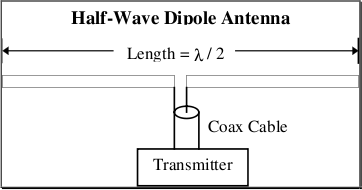
\includegraphics[scale=0.6]{figures/halfwave_antanna.png}\caption{\label{fig:halfwave}Half wave dipole (from \cite{primer})}
\end{figure}

This very simple antenna can be constructed by connection a simple wire. The length of the wire is half of the wavelength of the target carrier frequency. This so called half-wave dipole produces a radiation pattern as outlined in figure \ref{fig:halfwave_radiation}.

\begin{figure}[!h]
\centering
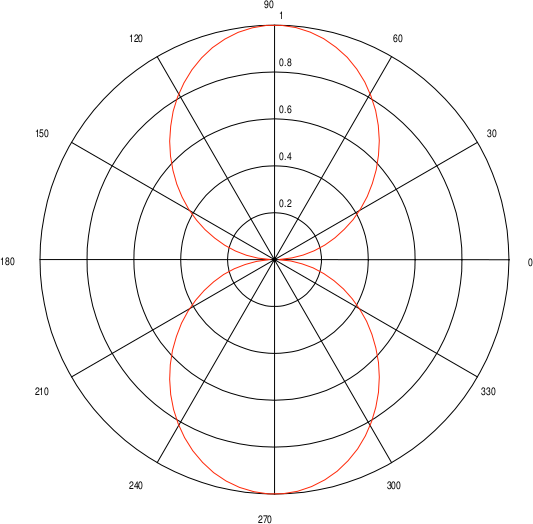
\includegraphics[scale=0.6]{figures/halfwave_radiation.png}\caption{\label{fig:halfwave_radiation}Half wave dipole radiaton (from \cite{primer})}
\end{figure}

\clearpage
\subsection{The line array antenna}
The radiation pattern as shown in figure \ref{fig:halfwave_radiation} shows two main reception directions heading at 90° and 270°. Furthermore one can observe a pretty wide radiation angle of about 120°. This simple dipole radiation pattern can be further improved by stacking many simple omni-directional antenna elements to an array of antennas as shown in figure \ref{fig:array}.

\begin{figure}[!h]
\centering
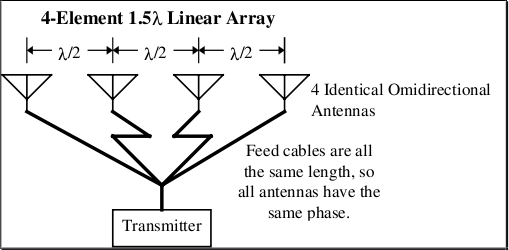
\includegraphics[scale=0.6]{figures/array_antenna.png}\caption{\label{fig:array}Linear array antenna (from \cite{primer})}
\end{figure}

When examining the radiation pattern of the linear array in figure \ref{fig:array_radiation} one can see that the radiation angle becomes much narrower. The directivity of this antenna is therefore much more focused to a specific target direction and much better helps to reduce the above mentioned effects of interference (by focusing to a specific direction) as well as amplifies the overall signal strength (by its gain).

\begin{figure}[!h]
\centering
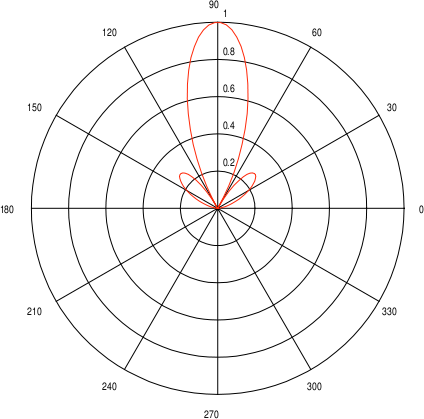
\includegraphics[scale=0.6]{figures/array_radiation.png}\caption{\label{fig:array_radiation}Line array antenna radiation (from \cite{primer})}
\end{figure}

One major problem of this antenna setup is that it is static due to its physical nature. One can place this kind of antenna in a way that a single "direction of interest" exists in order to improve general signal reception. This is possible in a setup where the transmitter and receiver both have static locations and don't move. But this assumption cannot be made in today's challenges of providing a flexible mobile wireless communication system.

\section{Beamforming}
A solution might be to rotate a directional antenna to the direction of interest mechanically. This method (although often being used) is too dependent on the availability of a mechanical rotor and causes a great deal of latency. This solution therefore is only suitable for very slowly moving direction targets. A much better solution is to control the angle of the direction pattern in a dynamic (electrical) way. Latency to target the direction of interest would be improved by a great amount of time and a mechanical rotor would not be needed at all.

The method of controlling the radiation pattern direction of a linear array antenna is called Beamforming. If the electric adjustment is done in a programmatic way this process is called "Digital Beamforming".\footnote{See \cite{primer}} The control of the radiation pattern in a linear array antenna can be achieved by adjusting the following two physical parameters of a signal being transmitted to or received from each array antenna element:

\begin{equation}
\begin{array}{ll}
a_k: & \textrm{The relative amplitude of the $k^{th}$ signal} \\
\theta_k: & \textrm{The phase shift of the $k^{th}$ signal} \\
\end{array}
\end{equation}

These parameters can be controlled in two ways:

\begin{itemize}
\item \emph{Electrically:} Phase and amplitude are controlled using electrical circuits.
\item \emph{DSP:} Phase and amplitude are controlled using digital signal processing algorithms.
\end{itemize}

From a computer scientist point of view the second solution is of particular interest. The mathematical background for these DSP algorithms is beyond the scope of this paper but essentially phase and amplitude can be combined using complex algebra. The combined variable includes imaginary parts and is being processed by algorithms. This variable $w_k$ is called the \emph{complex weight} of the $k^{th}$ antenna element:

\begin{equation}
\begin{array}{rcll}
w_k & = & a_k e^{i \sin(\theta_k)} & \textrm{where} \\
i & = & \sqrt{-1} & \textrm{(imaginary unit)} \\
\end{array}
\end{equation}

\clearpage
\subsection{Implementations}
Once the problem is solved on how to generate a desired radiation pattern and angle from a linear array antenna new challenges arise:

\begin{itemize}
\item How do we estimate the actual radiation direction?
\item How do we handle multiple access?
\end{itemize}

The above mentioned problems are being solved in solutions called "smart antennas". Even more sophisticated solutions like MIMO incorporate beamforming as one part of optimization techniques in order to achieve higher availability and throughput of wireless signals. These techniques are available in new wireless technologies like 802.11n and are being incorporated in newly available routers and access points.

One of the very many expected solutions on the market is the Ruckus 7962 access point. It implements beamforming algorithms in order to optimize the above mentioned challenges in WLAN access in large enterprises. One can see in figure \ref{fig:ruckus} how antennas are set up circularly in order to enhance the beamforming of radiation patterns.

\begin{figure}[!h]
\centering
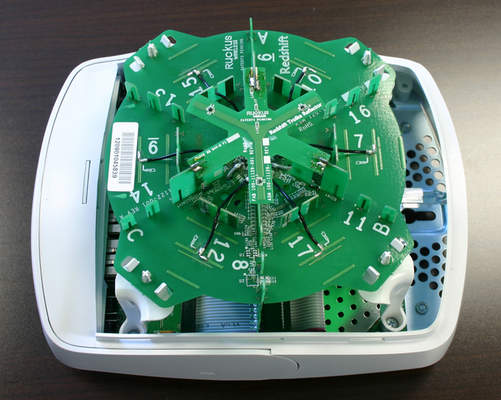
\includegraphics{figures/ruckus_7962.jpg}\caption{\label{fig:ruckus}Ruckus 7962 Access Point (from \cite{tomshardware})}
\end{figure}

This access point improves WLAN availability in areas with very high wireless usage such as in big enterprises. Figure \ref{fig:ruckus_wlan} illustrates the installation of such access points and their beamforming in a building.

\begin{figure}[!h]
\centering
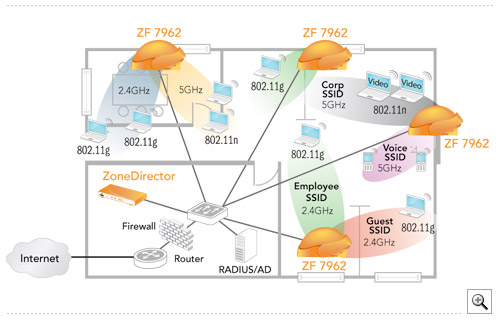
\includegraphics[scale=0.8]{figures/ruckus_wlan.jpg}\caption{\label{fig:ruckus_wlan}Ruckus WLAN installation (from \cite{ruckus})}
\end{figure}

\clearpage
\section{Conclusion}
One can see that beamforming is a very interesting and challenging technique for improving wireless technologies. The author encourages to perform basic simulations in existing scientific packages (Matlab, Octave, SciPy, etc.). Scripts were found on the internet but do not seem to be broadly enhanced and accessible.

Beamforming examples (esp. using DSP) for studying purposes therefore seem to be a very interesting task for further enhanced papers.
